\section{Results}

\subsection{Review-Based Branch}
The results for the general accuracy of each classifier is given in Figure \ref{accuracy}. We see that the highest accuracy achieved is 43.49\% by AdaBoost. We also see that, on average, the classifiers performed better when the features of adjective and adverb count were excluded.

\begin{figure}[!h]
\centering
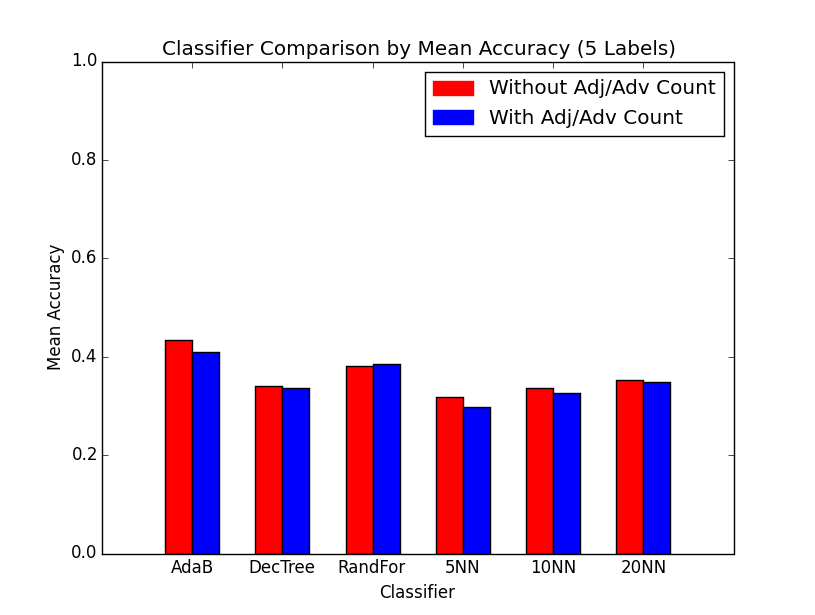
\includegraphics[scale=0.5]{compaccuracy}
\caption{}
\label{accuracy}
\end{figure}

The \texttt{scikit} package also provided a way of ranking the features by their importance when using Random Forest -- the more useful a feature was in making decisions (from the amount of variability in the feature), the higher the importance. It was found that the most important feature was the sentiment score, while the least important feature was the emphasized word count. Furthermore, the features of adjective and adverb count ranked fourth and fifth, which is unsurprising given the poorer classifier accuracy resulting from including those features.

We then explored the low classifier accuracies, specifically for AdaBoost, to see the distribution of correct and incorrect labels. Figure \ref{distribution} shows this distribution, plotting the frequencies of predicted-actual label pairs. The larger the point $(x,y)$, the more reviews labeled $y$ were predicted to be of class $x$. The points in red represent correctly-predicted reviews, as the predicted label matches with the actual label. From this, we can see that the classifier performed very well for five-star reviews (and was very close on four-star reviews), but also that the classifier predicted five stars for a large portion of reviews. This may also reflect an imbalance in the dataset. This imbalance can be seen in the star distribution of one of the datasets in Table \ref{rawdistribution}. Since each dataset was generated using the same process, this distribution is representative of each dataset. Clearly, the majority of the reviews in the dataset are five- and four-star reviews, which sheds light on the classifier performance in Figure \ref{distribution}. This distribution may also be unsurprising given the finding in \cite{imbalance} that people online tend to report positive emotions rather than negative emotions.

\begin{figure}[!h]
\centering
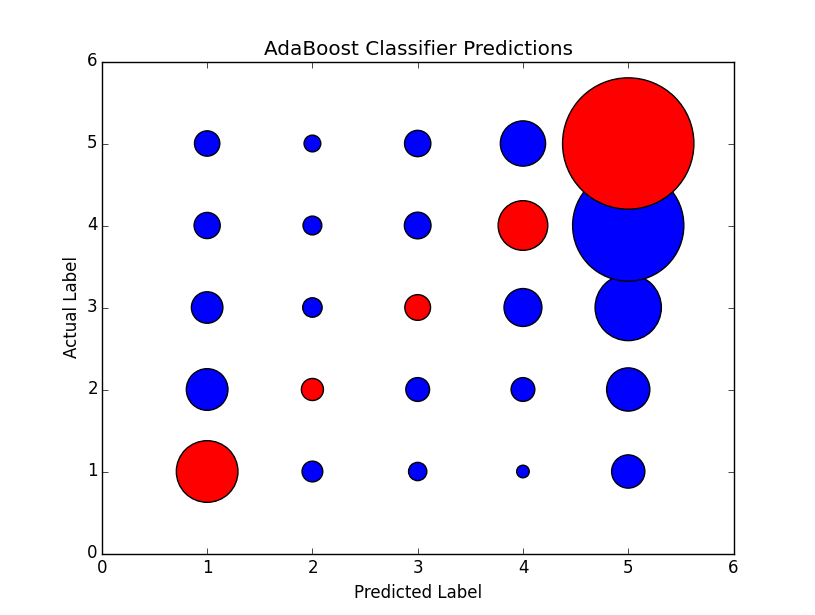
\includegraphics[scale=0.5]{ab_predict}
\caption{}
\label{distribution}
\end{figure}

\begin{table}[!h]
\centering
\caption{Star Distribution for One Dataset}
\label{rawdistribution}
\begin{tabular}{|r|c|c|c|c|c|}
\hline
\bf Rating & 1 & 2 & 3 & 4 & 5\\
\hline
\bf Percentage & 10.29\% & 8.98\% & 14.20\% & 29.44\% & 37.09\%\\
\hline
\end{tabular}
\end{table}

Figure \ref{extremes} shows the mean performance of the classifiers in determining whether or not the review is polarized (one- and five-star reviews vs. neither) on the left and the mean performance of the classifiers in determining whether or not the review is a five-star review on the right. Again, the inclusion of the adjective and adverb count features makes little difference in classifier performance; however, it did slightly increase the performance of the best classifier in this task -- Random Forest, which correctly predicted whether or not a review received five stars 59.99\% of the time. We can also see that the classifiers, on average, performed better at determining whether or not a review received five stars than determining whether or not a review was polarized, which may again be a manifestation of the star distribution in the dataset.

\begin{figure}[!h]
\centering
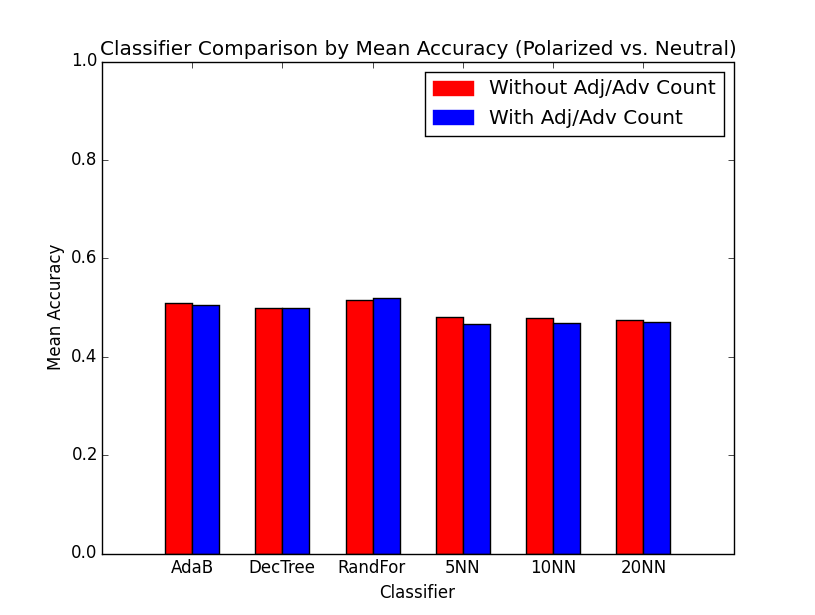
\includegraphics[scale=0.38]{compexaccuracy}
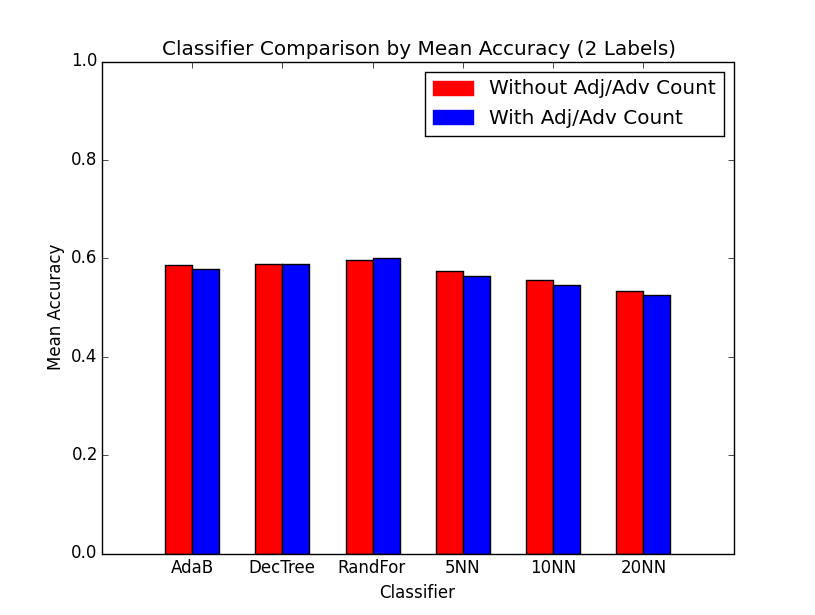
\includegraphics[scale=0.38]{compbinaccuracy}
\caption{}
\label{extremes}
\end{figure}

Finally, Figure \ref{offbyone} shows the mean ``soft'' accuracy of each classifier -- how often the classifier was at most one star away from the actual star rating of a review. AdaBoost performed the best again, correctly (and almost correctly) predicting the labels of 78.61\% of the reviews in the test set. Of course, we expect a higher accuracy in this task than in the original task of strictly correct label predictions, but we note that the performance is still better than the expected performance with random label assignments. If each review has a 20\% chance of being in one of the five classes, and if each review is randomly assigned a label as a prediction (each of which has a 20\% chance), then the expected ``soft'' accuracy is 52\%, so our classifiers still outperformed random assignment.

\begin{figure}[!h]
\centering
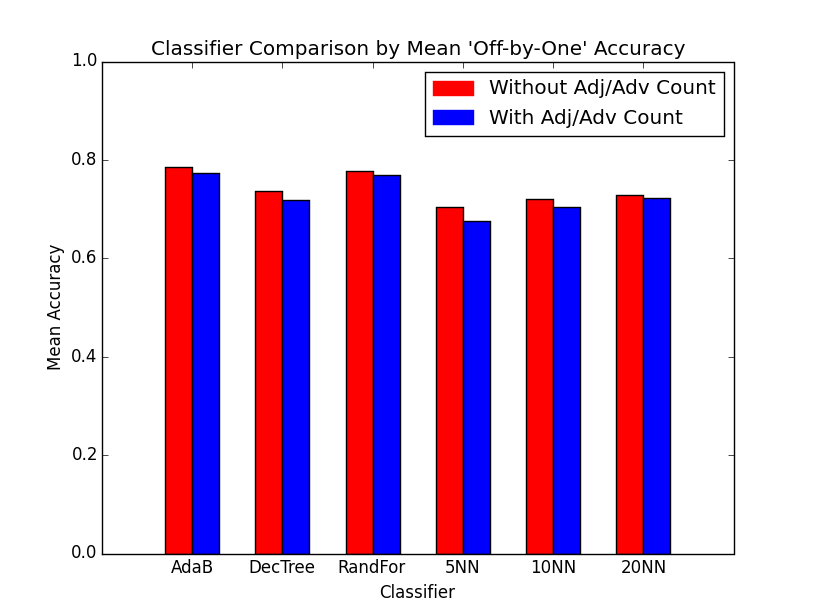
\includegraphics[scale=0.5]{compoffbyone}
\caption{}
\label{offbyone}
\end{figure}

\subsection{Profile-Based Branch}
\begin{itemize}
	\item RandomForest (all reviews)
	\begin{itemize}
		\item number of trees in the forest: 10
		\item minimum number of samples required to split an internal node: 1
		\item number of jobs is set to the number of cores: 4
		\item result: average cross validation score: 0.385 (3-fold)
	\end{itemize}
	\item SVC (support vector classifier) (10,000 reviews) \footnote{Due to the SVC function limitation in scikit-learn}
	\begin{itemize}
		\item Gaussian kernel: gamma (0.1), c(1)
		\item Gaussian, 45
		\item Linear c=1, 43 
		\item Polynomial degree 2, 44
		\item result: average cross validation score: 0.44 (3-fold)
	\end{itemize}
\begin{figure}[h]
\centering
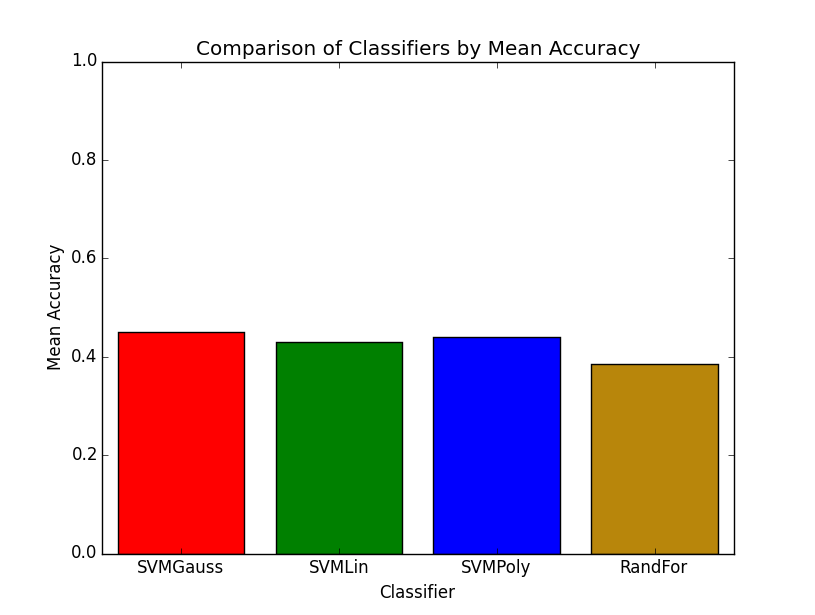
\includegraphics[width=0.5\linewidth]{profileaccuracy}
\caption{}
\label{fig:profileaccuracy}
\end{figure}

\end{itemize}




